\section{Gráfico da Função Logarítmica}
\begin{frame}
\frametitle{Gráfico da Função Logarítmica} 

\begin{exemplo}
Considere as funções logarítmicas tais que $f(x) = \log_2 x$ e $g(x)
= \log_{\frac 1 2} x$. Os gráficos de $f$ e $g$ são apresentados
abaixo.
\begin{center}
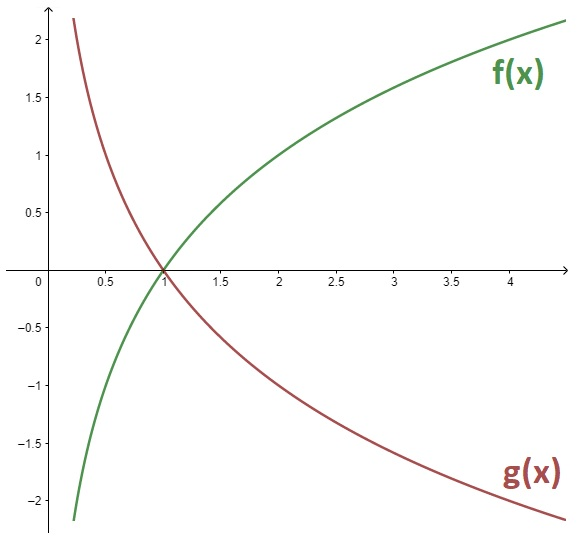
\includegraphics[width=6.1cm]{figures/graflog.jpg}
\end{center}
\end{exemplo}


\end{frame}

%------------------------------------------------------------------------------------------------------------

\begin{frame}
\frametitle{Gráfico da Função Logarítmica} 


Já vimos que o crescimento exponencial supera o de qualquer
polinômio. Por ser a inversa da função exponencial, a função
logarítmica possui um crescimento muito lento. Mesmo assim, a função
logarítmica é ilimitada superiormente. Compare os gráficos abaixo:
\begin{center}
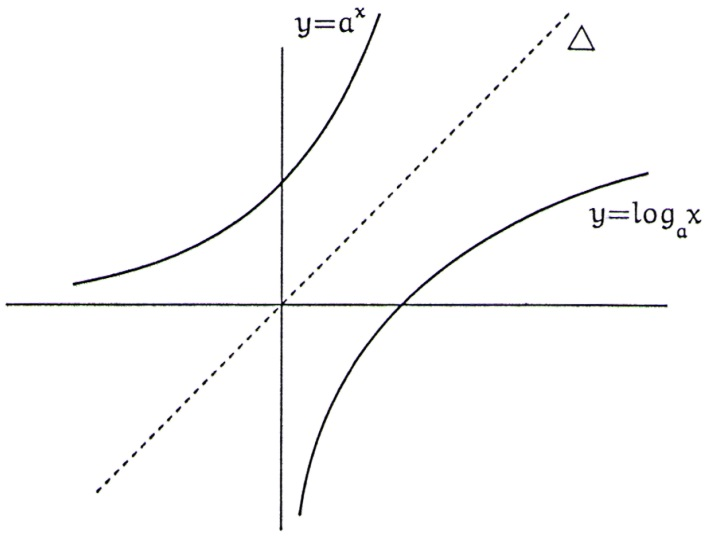
\includegraphics[width=7cm]{figures/logXexp.jpg}
\end{center}


\end{frame}
